\documentclass[a4paper,12pt]{report}

\usepackage{alltt, fancyvrb, url}
\usepackage{graphicx}
\usepackage[utf8]{inputenc}
\usepackage{hyperref}
\newcommand{\mail}[1]{\href{mailto:#1}{\texttt{#1}}}


\usepackage[italian]{babel}

\usepackage[italian]{cleveref}

\title{Relazione ``GSS'' \\ Gestionale Società Sportiva}

\author{Brini Tommaso (\mail{tommaso.brini@studio.unibo.it}) \\ Matricola 0000933814 \\ Mazzanti Gustavo (\mail{gustavo.mazzanti@studio.unibo.it}) \\ Matricola 0000914975 \\ Rambaldi Riccardo (\mail{riccardo.rambaldi4@studio.unibo.it}) \\ Matricola 0000875146}


\begin{document}

\maketitle

\tableofcontents

\chapter{Analisi dei requisiti}

Si vuole sviluppare un database a supporto della gestione di una società sportiva. La base di dati dovrà immagazzinare informazioni relative alla società in questione, ai tesserati e agli impegni in programma (allenamenti, partite, eventi vari). Il responsabile della società potrà quindi visualizzare tutti i giocatori, tutti i membri dello staff e tutti i dirigenti. Inoltre, potrà inserire nuovi eventi che verrano visualizzati in un calendario settimanale.

\section{Intervista}
Si vuole creare un gestionale per una società di calcio, di basket o di pallavolo. \newline
Si vuole innanzitutto tenere traccia delle informazioni della società, quali nome, sport, partita Iva, logo e colori sociali. \newline
Si vuole inoltre tenere traccia di tutti i tesserati della società sportiva, memorizzandone nome, cognome, codice fiscale, data di nascita, numero di matricola del tesserino, sesso, ruolo e eventualmente una foto di riconoscimento. \newline
Alla società appartengono diverse tipologie di persone: i giocatori, i membri dello staff e i dirigenti. I componenti delle prime due categorie devono appartenere a una categoria specifica (in altri termini, a una squadra). I dirigenti invece non appartengono a nessuna squadra. Ogni giocatore e ogni membro dello staff devono appartenere a una e una sola squadra, una singola persona perciò non può essere visualizzata in due categorie diverse. In aggiunta, per i giocatori è necessario salvare anche peso, altezza, la data di scadenza del certificato medico e la mano/piede preferito (a seconda dello sport selezionato). \newline
Per ogni persona ci deve essere la possibilità di salvare dei documenti visualizzabili nella scheda della persona stessa. \newline
Si vuole infine visualizzare in un calendario tutti gli impegni della società. Gli impegni possono essere di tre tipi: partite, allenamenti o eventi generici (a cui verrà assegnata una breve descrizione). A ogni partita e a ogni allenamento può partecipare solo una squadra, mentre per gli eventi generici è necessario creare una lista di convocati.


\section{Estrazione dei concetti principali}
A seguito della lettura e comprensione dei requisiti richiesti dal cliente, si procede sviluppando un testo che ne riassuma tutti i concetti principali. 
Si tiene conto delle seguenti correzioni di ambiguità.

\begin{figure}[htp]
    \centering
    \includegraphics[width = \textwidth]{GSS_report/img/ambiguità.png}
    \caption{Rilevamento delle ambiguità e correzioni proposte}
    \label{fig:umlAnalisys}
\end{figure}

L'applicazione vuole gestire una sola \textbf{Società} sportiva, scegliendo lo \textbf{Sport} tra calcio, basket o pallavolo. \newline
Innanzitutto, bisogna salvare le informazioni della società, quali nome, sport, partita Iva, colori sociali e un'\textbf{Immagine} associata. \newline
Alla società appartengono tre tipi di \textbf{Persone}: \textbf{Giocatore}, \textbf{Staff} e \textbf{Dirigente}. Per ogni persona va salvato nome, cognome, codice fiscale, data di nascita, numero di matricola del tesserino, sesso, ruolo e eventualmente un'immagine associata. \newline
I giocatori e lo staff appartengono a una specifica \textbf{Categoria}, mentre i dirigenti non appartengono a nessuna categoria. La società può avere infinite categorie.
Ogni persona può appartenere a una e una sola categoria. \newline
Per i giocatori è necessario salvare anche peso, altezza, la data di scadenza del certificato medico e la preferenza. \newline
Per ogni persona si può caricare nel database delle immagini relative ai vari documenti personali.
\newline
Si vuole infine tenere un calendario degli \textbf{Eventi}. Gli eventi da tenere in considerazione sono \textbf{Partita}, \textbf{Allenamento} ed \textbf{Evento Generico}. A quest'ultimo verrà assegnato un nome o una breve descrizione. \newline
A ogni allenamento e a ogni partita può partecipare una sola categoria. Per gli eventi generici è necessario creare una lista di convocati, scelti tra tutte le persone tesserate alla società.

\section{Elenco delle azioni principali}
\begin{itemize}
    \item Creazione di una nuova società con realtivo logo, nome, colori sociali, partita Iva e lo sport di riferimento,
    \item Creazione di una nuova categoria,
    \item Creazione di una nuova persona (Giocatore, Dirigente o Staff),
    \item Creazione di un nuovo evento con le relative convocazioni (Allenamento, Partita o Evento Generico),
    \item Visualizzazione di tutte le categorie,
    \item Visualizzazione di una singola categoria (elenco Giocatori e Staff) oppure la categoria Dirigenti,
    \item Visualizzazione scheda singola persona,
    \item Inserimento e visualizzazione documenti della persona,
    \item Modifica del risultato negli eventi di tipo Partita,
    \item Visualizzazione del calendario settimanale,
    \item Visualizzazione singolo evento,
    \item Visualizzazione convocati all'evento,
    \item Eliminazione della singola persona, con conseguente eliminazione dei documenti e delle convocazioni relative,
    \item Eliminazione del singolo evento, con conseguente eliminazione delle convocazioni relative.
\end{itemize}


\chapter{Progettazione concettuale}
\section{Società}
\subsection{Progettazione dello schema E/R}
Lo schema scheletro della società comprende la principali entità in diretta relazione con essa.
\newline
\begin{figure}[htp]
    \centering
    \includegraphics[width = \textwidth]{GSS_report/img/società.png}
    \caption{Schema scheletro della Società}
\end{figure}
\subsection{Raffinamenti proposti}
L'entità \textbf{Società} deve avere una partita IVA che la identifica in modo univoco nel caso in cui, in un'ottica futura di aggiornamento, si volessero aggiungere più società al database. Inoltre, la \textbf{Società} deve avere un nome (non necessariamente univoco), due \textbf{colori sociali} (che l'utente potrà scegliere al primo avvio del programma) e infine uno stemma, rappresentato come \textbf{Immagine} (nel caso in cui non v engsa caricato uno stemma ne verrà inserito uno di default) in relazione 1-N \textbf{Rappresenta} con \textbf{Società}. \newline \newline
Per quanto riguardo lo \textbf{Sport}, vista la necessità di popolare le tabelle dei ruoli dei giocatori a seconda dello sport scelto, abbiamo creato una relazione 1-N \textbf{Pratica} tra \textbf{Società} e \textbf{Sport}.
\begin{figure}[htp]
    \centering
    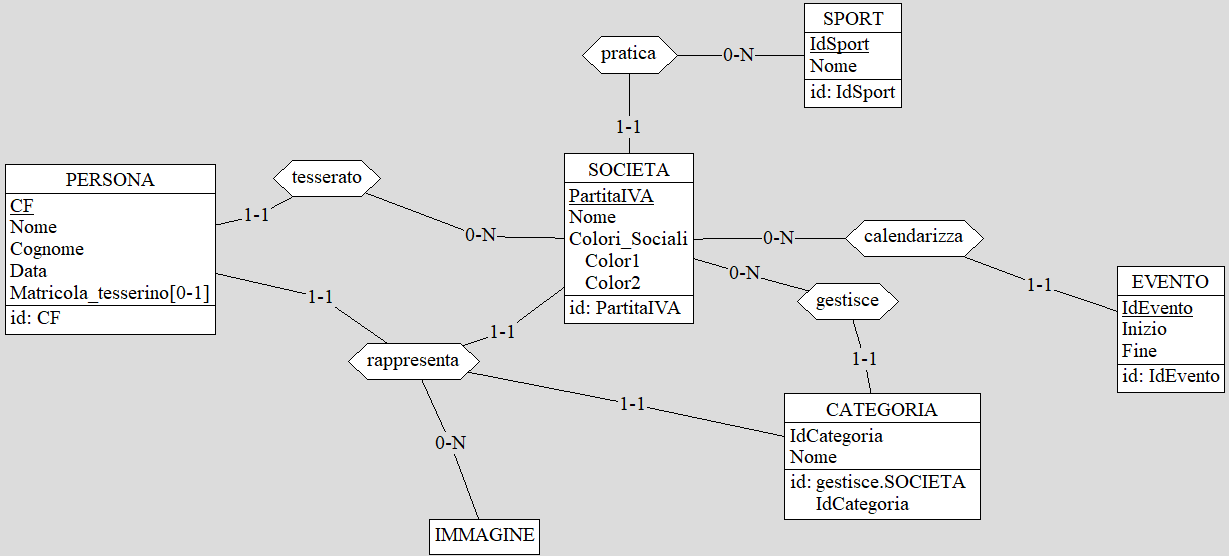
\includegraphics[width = \textwidth]{GSS_report/img/societa_raffinamento.png}
    \caption{Schema E/R parziale della Società}
\end{figure}

\newpage
\section{Persona}
\subsection{Progettazione dello schema E/R}
Lo schema scheletro della Persona comprende la principali entità in diretta relazione con essa.
\begin{figure}[htp]
    \centering
    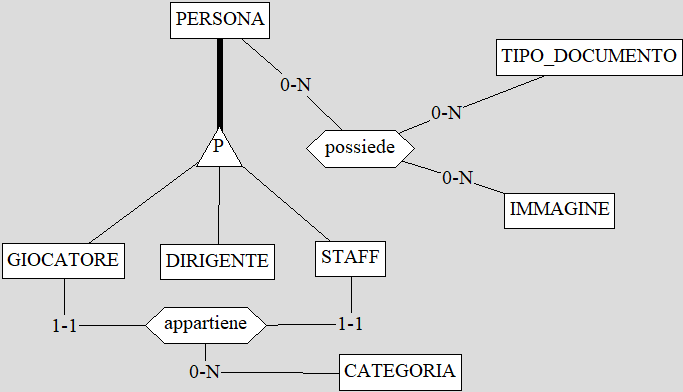
\includegraphics[width = \textwidth]{GSS_report/img/persona.png}
    \caption{Schema scheletro della Persona}
\end{figure}
\subsection{Raffinamenti proposti}
Una \textbf{Società} sportiva è composta da più persone (tesserate) che ricoprono vari ruoli.
Per evitare ridondanze, l'entità \textbf{Persona} è stata specializzata delle tre entità \textbf{Giocatore}, \textbf{Dirigente} e \textbf{Staff} che ereditano da \textbf{Persona} l'identificatore  \textbf{CF}, il \textbf{Nome}, il \textbf{Cognome} e la \textbf{Data} di nascita.
Questa generalizzazione è totale ed esclusiva; in questo senso, una persona può essere o un \textbf{Giocatore} o un \textbf{Dirigente} o far parte dello \textbf{Staff}, e non può essere altrimenti. \newline \newline
Ogni persona può essere rappresentata da una foto (in caso contrario ne viene caricata una di default) e possiede un documento sotto forma di immagine di cui viene specificata anche la tipologia (es. carta d'identità) in \textbf{Tipo Documento}, di conseguenza \textbf{Persona} possiede due relazioni differenti con \textbf{Immagine}: una 1-N \textbf{Rappresenta} e una 0-N \textbf{Possiede}. \newline \newline
Sia \textbf{Staff}, \textbf{Giocatore} e \textbf{Dirigente} devono ricoprire ognuno un determinato ruolo, ma solo \textbf{Staff} e \textbf{Giocatore} devono far parte di una e soltanto una \textbf{Categoria}. Ogni ruolo ha un identificatore e una breve \textbf{Descrizione}.
Alla creazione del database verranno popolate le tabelle \textbf{Sesso}, \textbf{Mano Piede Preferito}, \textbf{RuoloStaff} e \textbf{RuoloDirigente}, mentre la tabella \textbf{RuoloGiocatore} verrà popolata solo in base alla scelta dello sport alla creazione della società.
\begin{figure}[htp]
    \centering
    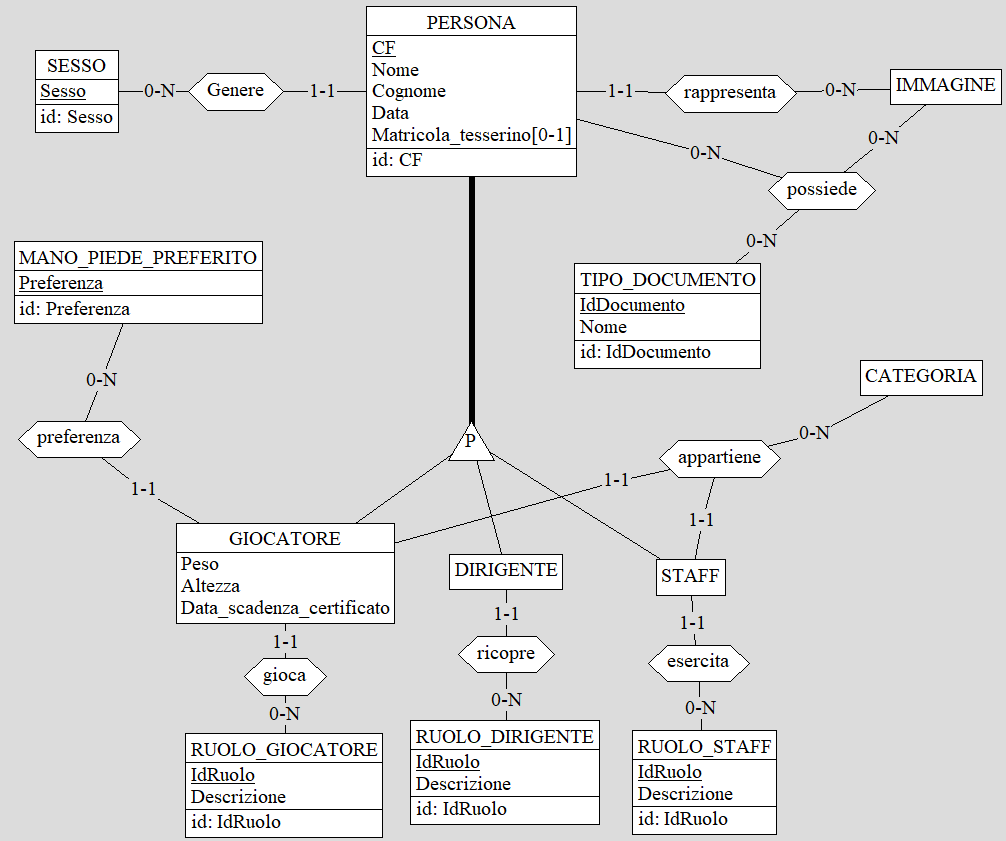
\includegraphics[width = \textwidth]{GSS_report/img/persona_raffinamento}
    \caption{Schema E/R parziale della Persona}
\end{figure}

\newpage
\section{Categoria}
\subsection{Progettazione dello schema E/R}
Lo schema scheletro della Categoria comprende la principali entità in diretta relazione con essa.
\begin{figure}[htp]
    \centering
    \includegraphics[width = \textwidth]{GSS_report/img/categoria.png}
    \caption{Schema scheletro della Categoria}
\end{figure}
\subsection{Raffinamenti proposti}
Una \textbf{Categoria} all'interno di una società sportiva è una squadra composta da giocatori (di una determinata età) e da un rispettivo staff.
Ogni \textbf{Categoria} ha un identificatore numerico incrementale e un \textbf{Nome}; Inoltre, possiede un'\textbf{Immagine} (tipicamente una foto della squadra) e può disputare partite e allenamenti .
\begin{figure}[htp]
    \centering
    \includegraphics[width = \textwidth]{GSS_report/img/categoria_raffinamento.png}
    \caption{Schema E/R parziale della Categoria}
\end{figure}

\newpage
\section{Evento}
\subsection{Progettazione dello schema E/R}
Lo schema scheletro dell'Evento comprende la principali entità in diretta relazione con esso.
\begin{figure}[htp]
    \centering
    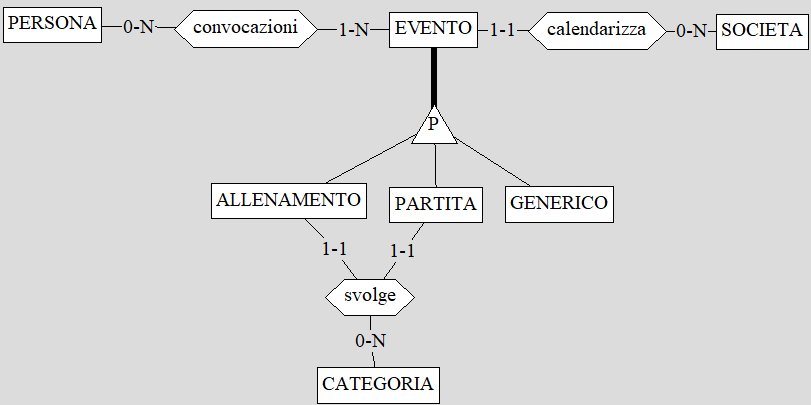
\includegraphics[width = \textwidth]{GSS_report/img/evento.png}
    \caption{Schema scheletro dell'Evento}
\end{figure}
\subsection{Raffinamenti proposti}
\begin{figure}[htp]
    \centering
    \includegraphics[width = \textwidth]{GSS_report/img/categoria_raffinamento.png}
    \caption{Schema E/R parziale dell'Evento}
\end{figure}
\newpage
\section{Schema Finale}

\chapter{Progettazione logica}
\section{Stima del volume dei dati}
\section{Descrizione delle operazioni principali}
\section{Tabelle degli accessi}
\section{Raffinamento dello schema}
\section{Analisi delle ridondanze}
\section{Schema relazionale finale}
\section{Traduzione delle operazioni in query SQL}

\chapter{Progettazione dell'applicazione}
\section{Descrizione dell'architettura}
Si sviluppa una applicazione molto semplice per la gestione del database in linguaggio Java, che renda 
possibile la messa in pratica delle operazioni richieste dalle varie viste. L’approccio verso il DB è gestito 
tramite JDBC. Il DB risiede in locale e usa MySQL Server come DBMS.  
Per ogni tabella contenuta nel DB viene creata una corrispettiva classe che la rappresenta all’interno del 
model dell’applicazione, tutte queste classi estendono una classe univoca chiamata Entity tramite la quale
sarà possibile implementare dei metodi univoci per tutte le entità come il metodo di inserimento e cancellazione sul DB,
in alcune classi finali, come \textbf{Person, Event...}, sono stati sovrascritti alcuni metodi comuni per poter adattare
meglio la classe alla struttura del DB.
Tutte le query utili per inserimento, modifica, visulizzazione e cancellazione si troveranno all'interno di una classe
statica chiamata \textbf{Utilities}.
Al primo avvio viene proposta una schermata iniziale che richiederà le informazioni della società, come
\textbf{nome della società, Partita Iva, colori sociali, lo sport di riferimento ed eventualmente un logo} (La scelta dei colori
potrà essere evitata scegliendo in entrambi i campi il colore "White", il sistema in questo caso inserirà i colori di default),
una volta terminato l'inserimento della società, la classe Society si occuperà di popolare la tabella con i dati appena inseriti
all'interno del DB e conseguentemente, in base allo sport selezionato, verrà riempita la tabella \textbf{ruolo giocatore} con i ruoli predefiniti.
\begin{figure}[htp]
    \centering
    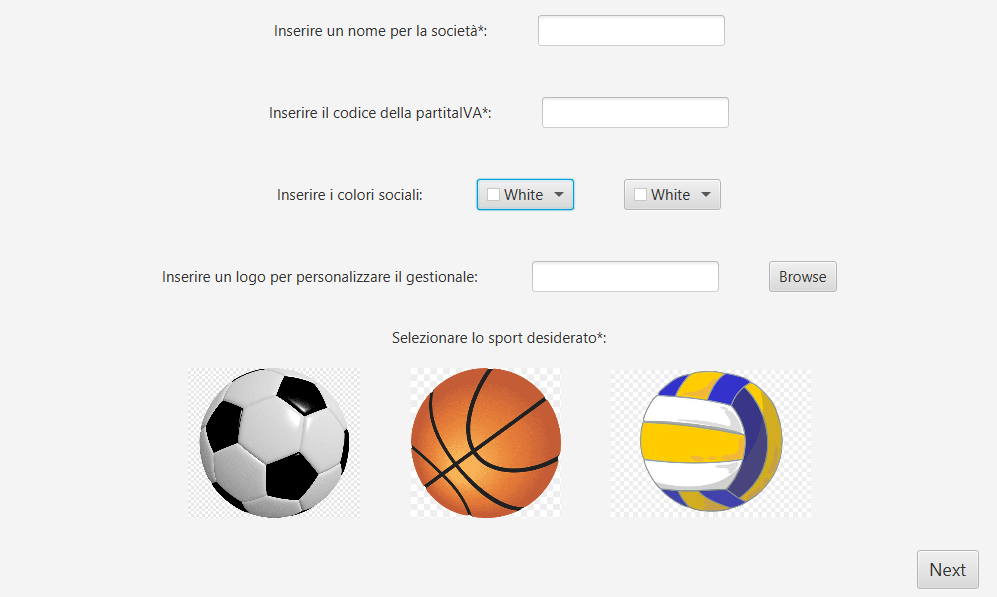
\includegraphics[width = \textwidth]{GSS_report/img/schermata_iniziale.png}
    \caption{Schermata iniziale di inserimento della categoria}
    \label{fig:umlAnalisys}
\end{figure}

\newpage
Una volta terminata l'operazione di primo avvio, si presenterà la schermata home del programma, quella che si presenterà a tutti i successivi
avvii successivi al primo.
La schermata home si presenterà con una doppia scheda, la prima mostrerà a video tutte le categorie inserite, oltre alla "categoria" \textbf{Dirigenti},
la quale conterrà tutte le persone iscritte che non hanno una vera e propria categoria, oltre ai bottoni per 
Nella seconda scheda, tramite un menu a schede, sarà possibile spostarsi nella visualizzazione del calendario, il quale presenterà
la settimana corrente ma con la possibilità di vedere le settimane passate e future.
Il login vero e proprio con inserimento di id e password non viene gestito poiché le password non vengono memorizzate nel DB. 
Viene effettuata però una cosa molto simile, infatti nel caso del login di un dipendente esso deve 
specificare il suo id univoco. La correttezza di tale inserimento viene confermata se viene inserito un id che 
effettivamente è presente nel database. In tal caso tutte le operazioni che vengono effettuate da quel 
momento in poi, vengono registrate con autore: quel dipendente. Nel caso invece volesse accedere 
l’amministratore, egli dovrebbe specificare una password che solo lui conosce. A quel punto avrebbe 
accesso alla schermata di amministrazione, in cui potrebbe eseguire le operazioni da lui richieste.

\bibliographystyle{alpha}
\bibliography{13-template}

\end{document}
